\documentclass{article}

% if you need to pass options to natbib, use, e.g.:
%     \PassOptionsToPackage{numbers, compress}{natbib}
% before loading neurips_2026

% The authors should use one of these tracks.
% Before accepting by the NeurIPS conference, select one of the options below.
% 0. "default" for submission
\usepackage[preprint]{neurips_2026}
% the "default" option is equal to the "main" option, which is used for the Main Track with double-blind reviewing.
% 1. "main" option is used for the Main Track
%  \usepackage[main]{neurips_2026}
% 2. "position" option is used for the Position Paper Track
%  \usepackage[position]{neurips_2026}
% 3. "eandd" option is used for the Evaluations & Datasets Track
 % \usepackage[eandd]{neurips_2026}
 % if you want to opt-in for a de-anomymized submission (not recommended, but OK):
 %\usepackage[eandd, nonanonymous]{neurips_2026}
% 4. "creativeai" option is used for the Creative AI Track
%  \usepackage[creativeai]{neurips_2026}
% 5. "sglblindworkshop" option is used for the Workshop with single-blind reviewing
 % \usepackage[sglblindworkshop]{neurips_2026}
% 6. "dblblindworkshop" option is used for the Workshop with double-blind reviewing
%  \usepackage[dblblindworkshop]{neurips_2026}

% After being accepted, the authors should add "final" behind the track to compile a camera-ready version.
% 1. Main Track
 % \usepackage[main, final]{neurips_2026}
% 2. Position Paper Track
%  \usepackage[position, final]{neurips_2026}
% 3. Evaluations & Datasets Track
 % \usepackage[eandd, final]{neurips_2026}
% 4. Creative AI Track
%  \usepackage[creativeai, final]{neurips_2026}
% 5. Workshop with single-blind reviewing
%  \usepackage[sglblindworkshop, final]{neurips_2026}
% 6. Workshop with double-blind reviewing
%  \usepackage[dblblindworkshop, final]{neurips_2026}
% Note. For the workshop paper template, both \title{} and \workshoptitle{} are required, with the former indicating the paper title shown in the title and the latter indicating the workshop title displayed in the footnote.
% For workshops (5., 6.), the authors should add the name of the workshop, "\workshoptitle" command is used to set the workshop title.
% \workshoptitle{WORKSHOP TITLE}

% "preprint" option is used for arXiv or other preprint submissions
 % \usepackage[preprint]{neurips_2026}

% to avoid loading the natbib package, add option nonatbib:
%    \usepackage[nonatbib]{neurips_2026}

\usepackage[utf8]{inputenc}      % allow utf-8 input
\usepackage[T1]{fontenc}         % use 8-bit T1 fonts
\usepackage{hyperref}            % hyperlinks
\usepackage{url}                 % simple URL typesetting
\usepackage{booktabs}            % professional-quality tables
\usepackage{amsfonts}            % blackboard math symbols
\usepackage{amsmath}             % advanced math
\usepackage{graphicx}            % figure inclusion
\usepackage{nicefrac}            % compact symbols for 1/2, etc.
\usepackage{microtype}           % microtypography
\usepackage{xcolor}              % colors

\bibliographystyle{plainnat}

\title{Lab 1: CIFAR-10 Classification with LeNet-5 and ResNet-Based CNN}


\author{
  Yong Cuiyang\\
  21307140051\\
  School of Data Science\\
  Fudan University\\
}


\begin{document}


\maketitle


\begin{abstract}
  This report systematically evaluates convolutional neural networks (CNNs) on the CIFAR-10 image classification benchmark. 
  We first train a baseline LeNet-5 and examine its overfitting behaviour, 
  then introduce L2 regularization and Dropout in an attempt to mitigate it. 
  A comprehensive hyperparameter search over learning rate, weight decay, label smoothing, 
  and batch size is conducted to study their marginal and interaction effects. 
  Finally, we implement a modern CNN (MyCNN) adapted from ResNet-18 for 32$\times$32 inputs 
  and compare its performance against the LeNet variants. 
  Results show that while mild regularisation improves calibration, 
  it reduces the test accuracy of the small-capacity LeNet-5 from 68.02\% to 65.01\%. 
  Hyperparameter tuning through a 54-experiment grid search identifies an optimal combination achieving 71.40\% test accuracy. 
  The ResNet-based MyCNN, trained with stronger data augmentation and cosine annealing scheduling, 
  substantially outperforms all LeNet models with a test accuracy of 95.04\%\footnote{Code, model weights, and training logs are available on \href{https://github.com/Snivallus/Introduction-to-AI-Project-01}{Snivallus/Introduction-to-AI-Project-01}.}.
\end{abstract}


\section{Introduction}\label{sec:introduction}

Image classification is a fundamental task in computer vision, 
and convolutional neural networks (CNNs) have been the dominant approach 
since the pioneering work of LeNet-5 \citep{lecun1998gradient} for handwritten digit recognition. 
Subsequent advances such as AlexNet, VGG, and ResNet \citep{he2016deep} 
have progressively pushed the state of the art on large-scale benchmarks, 
demonstrating the importance of depth, skip connections, and regularisation techniques.

The CIFAR-10 dataset \citep{krizhevsky2009learning} provides a suitable benchmark for educational experimentation: 
it contains 60\,000 32$\times$32 colour images across 10 balanced classes, 
with a standard 50\,000/10\,000 train/test split. 
Its moderate resolution and class balance make it well-suited for systematically studying overfitting, 
regularisation, and the effect of architectural capacity on generalisation.

This report presents four experimental tasks: 
(1) training a baseline LeNet-5 and analysing its overfitting behaviour; 
(2) introducing L2 weight decay and Dropout to regularise the model; 
(3) conducting a 4-factor grid search over learning rate, weight decay, label smoothing, and batch size; 
and (4) implementing a modern ResNet-style CNN (MyCNN) and comparing its performance against the LeNet variants. 
All experiments are conducted using PyTorch with a shared training pipeline that includes cosine annealing with warm restarts and early stopping.


\section{Methods}\label{sec:methods}

\subsection{CIFAR-10 Dataset}\label{subsec:cifar-10-dataset}

CIFAR-10 consists of 60\,000 32$\times$32 RGB images partitioned into 10 classes: 
airplane, automobile, bird, cat, deer, dog, frog, horse, ship, and truck. 
The training set contains 50\,000 images (5\,000 per class) 
and the test set contains 10\,000 images (1\,000 per class). 
The dataset is perfectly balanced, as shown in Figure~\ref{fig:data-class-dist}. 
For our experiments, we further split the training set into 45\,000 training samples 
and 5\,000 validation samples using a fixed random seed.

\begin{figure}[tbp]
  \centering
  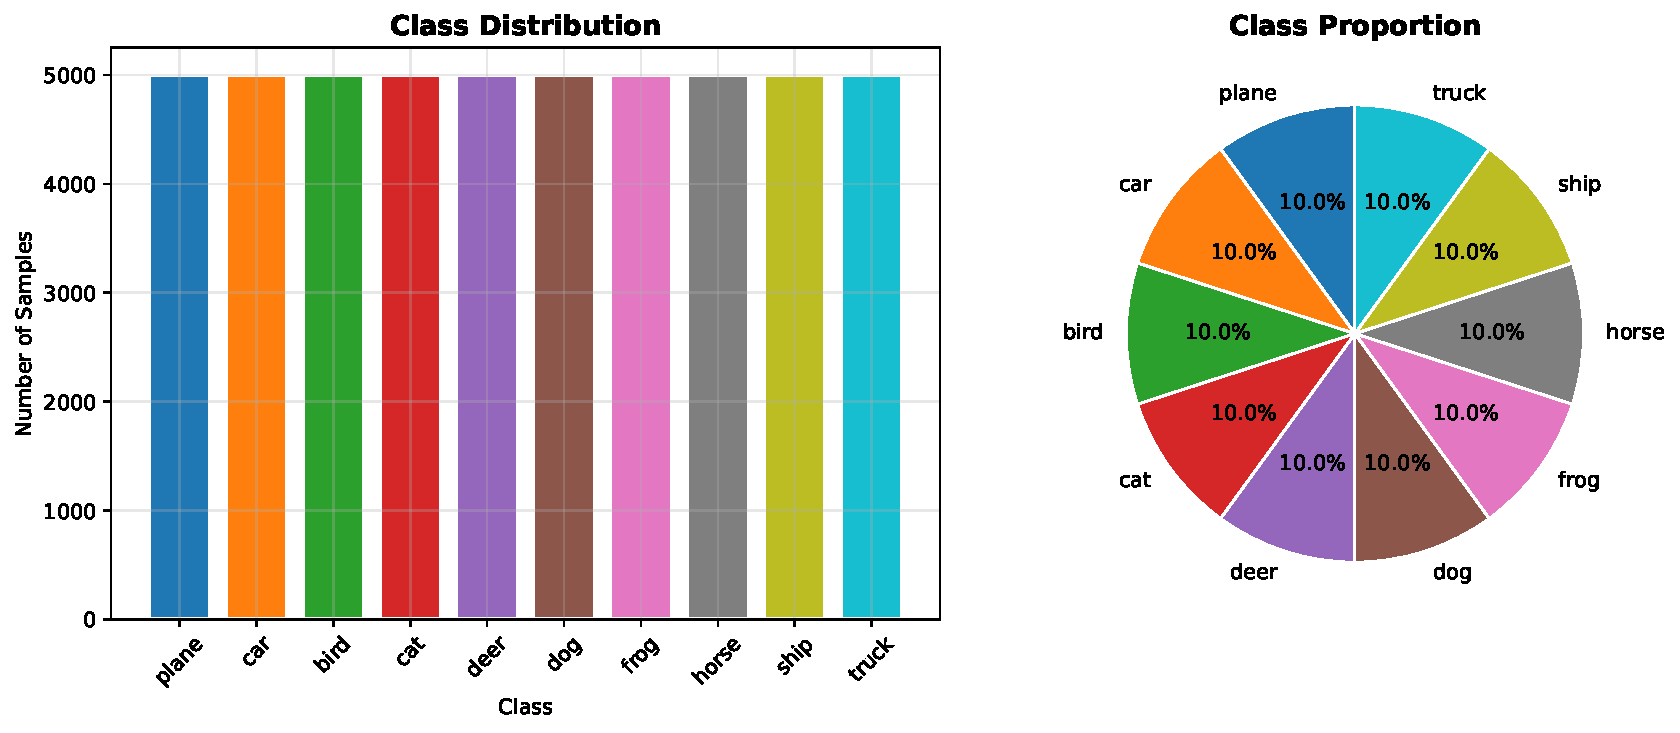
\includegraphics[width=0.85\textwidth]{../figures/data_exploration_class_distribution.pdf}
  \caption{Class distribution of the CIFAR-10 training set. Each of the 10 classes contains exactly 5\,000 samples, confirming the balanced nature of the dataset.}
  \label{fig:data-class-dist}
\end{figure}

Figure~\ref{fig:sample-grid} shows five example images per class, 
illustrating the visual diversity within each category. 
Per-channel pixel statistics (Table~\ref{tab:pixel-stats}) reveal that the blue channel has a slightly lower mean, 
which informs the normalisation strategy applied in all experiments.

\begin{figure}[tbp]
  \centering
  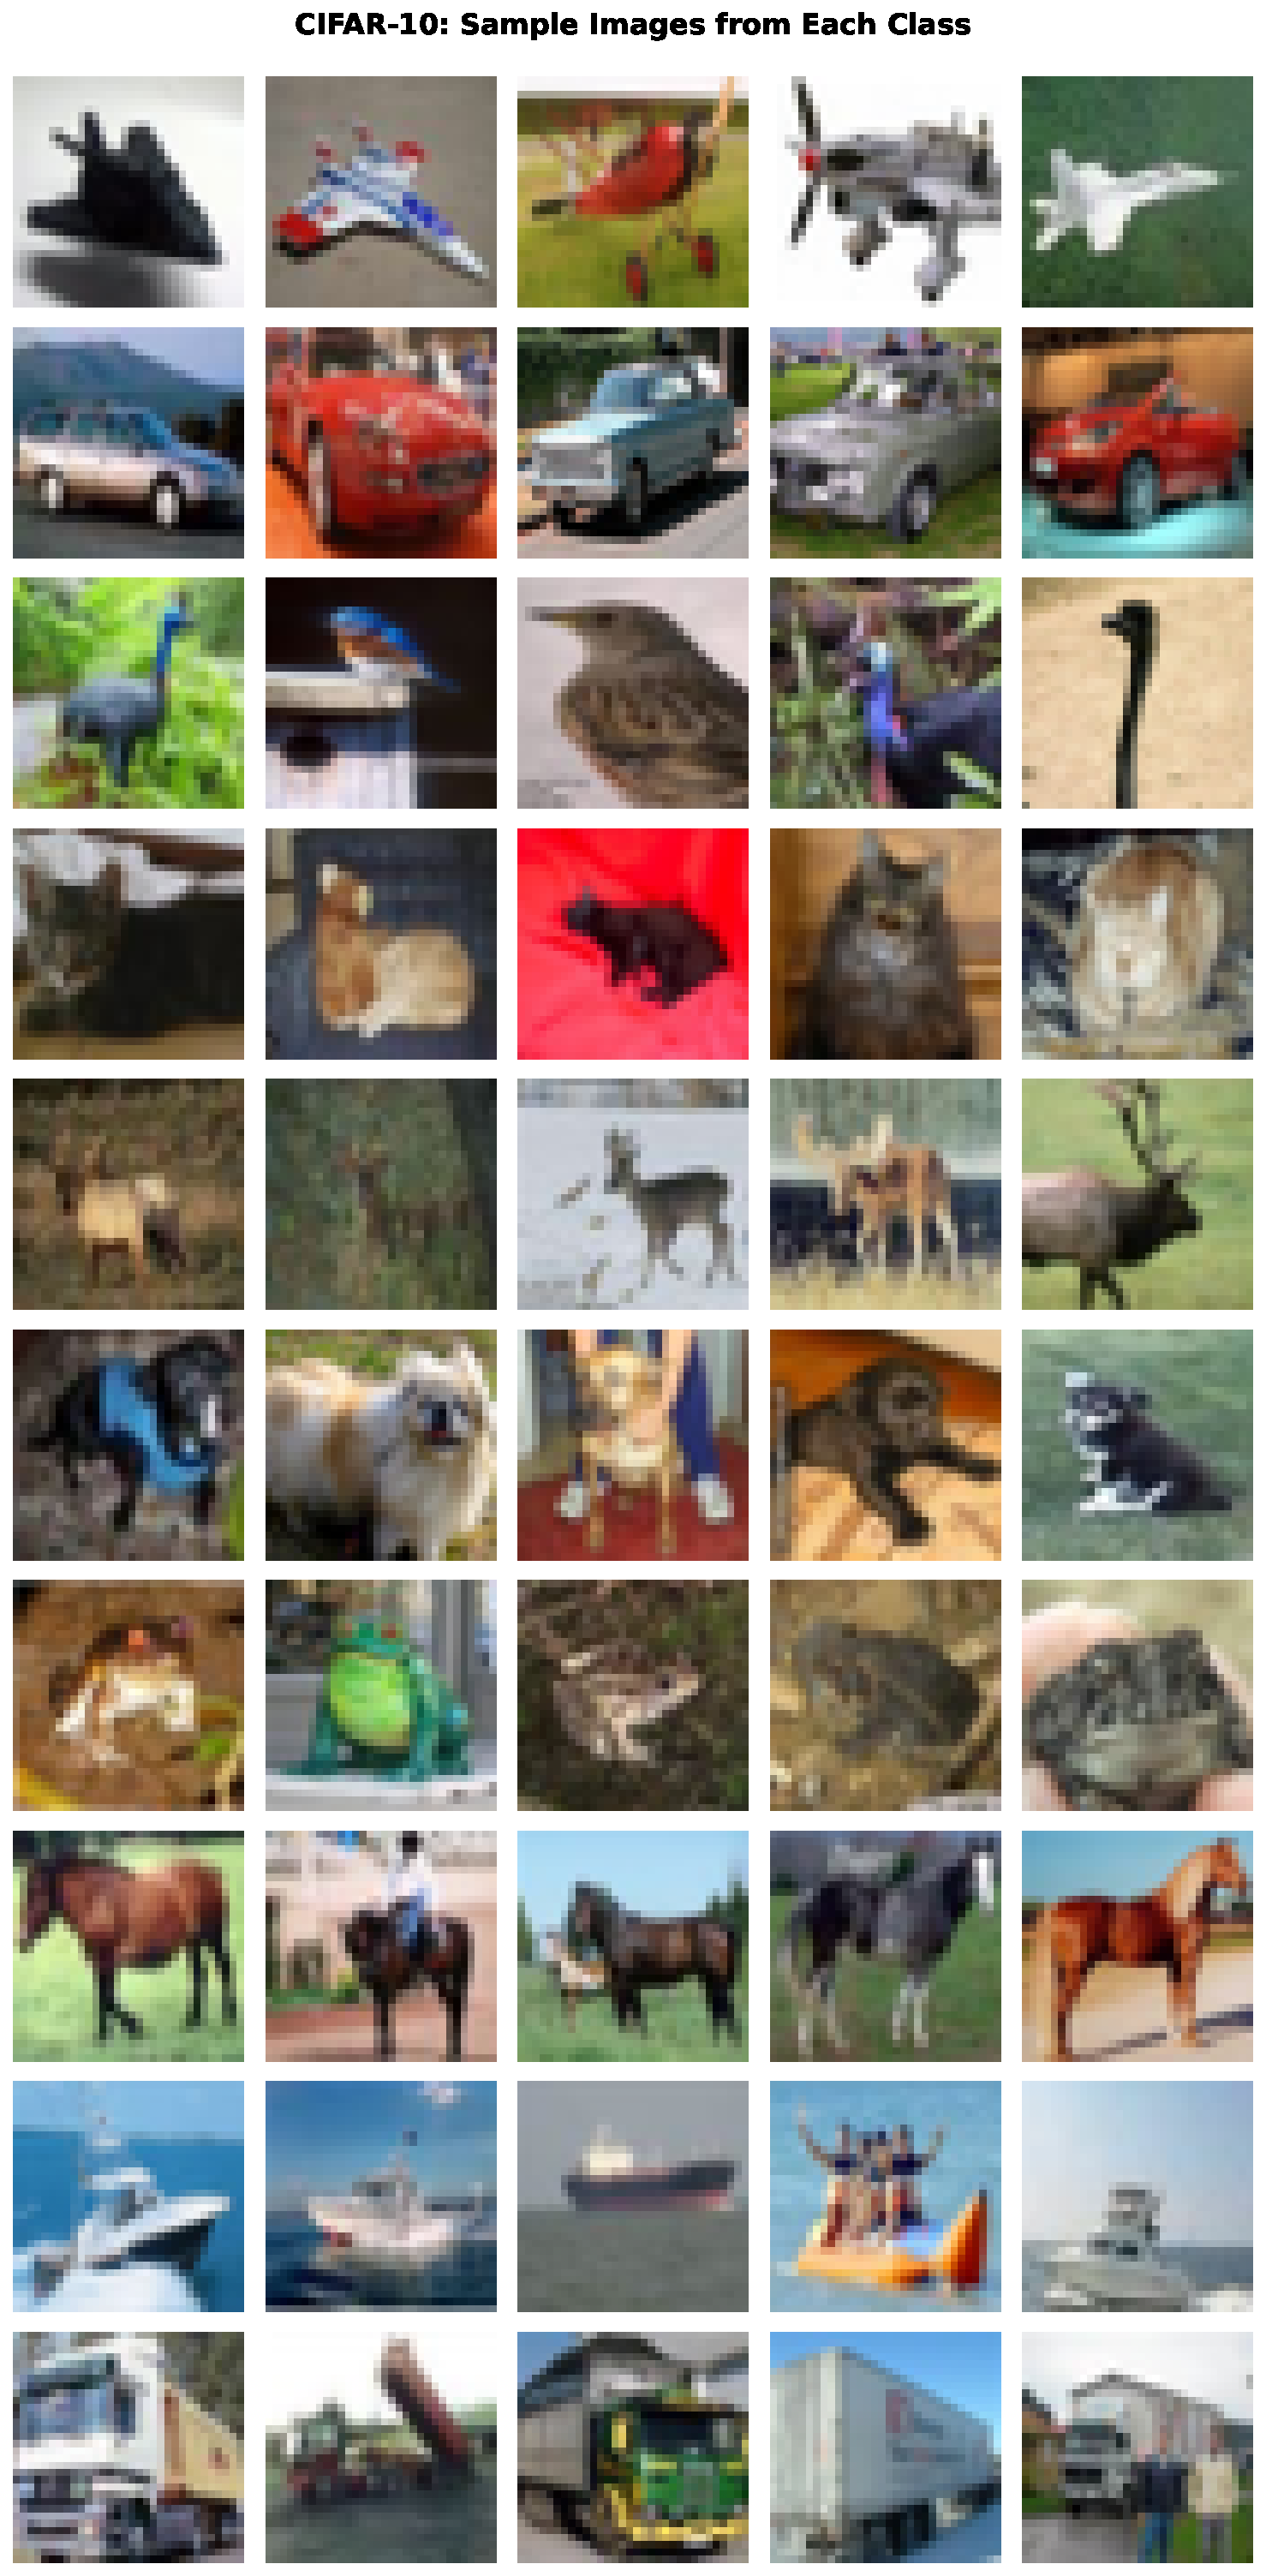
\includegraphics[width=0.75\textwidth]{../figures/data_exploration_sample_grid.pdf}
  \caption{Sample images from each CIFAR-10 class. The dataset captures natural images with varying backgrounds, poses, and lighting conditions.}
  \label{fig:sample-grid}
\end{figure}

\begin{table}[t]
  \centering
  \caption{Per-channel pixel statistics for the CIFAR-10 training set (raw pixel values in $[0, 1]$).}
  \label{tab:pixel-stats}
  \begin{tabular}{lccccc}
    \toprule
    Channel & Mean & Std & Min & Max \\
    \midrule
    Red   & 0.4914 & 0.2470 & 0.0 & 1.0 \\
    Green & 0.4822 & 0.2435 & 0.0 & 1.0 \\
    Blue  & 0.4465 & 0.2616 & 0.0 & 1.0 \\
    \bottomrule
  \end{tabular}
\end{table}


\subsection{Data Augmentation}\label{subsec:data-augmentation}

Two levels of data augmentation are employed, implemented in the \path{get_cifar10_data_augmentation()} function. 
The \emph{light} augmentation (used for LeNet-5 experiments) applies random horizontal flips with probability 0.1 
and random crops with padding of 4 pixels (also with probability 0.1). 
The \emph{full} augmentation (used for MyCNN) additionally applies colour jittering (brightness, contrast, saturation, hue), 
Gaussian blur, small rotations ($\pm 5^\circ$), and random erasing, all with probability 0.2 (see Figure~\ref{fig:augmentation}). 
The test transform is identical in both cases: ToTensor followed by normalisation using the per-channel mean and standard deviation from Table~\ref{tab:pixel-stats}.

\begin{figure}[tbp]
  \centering
  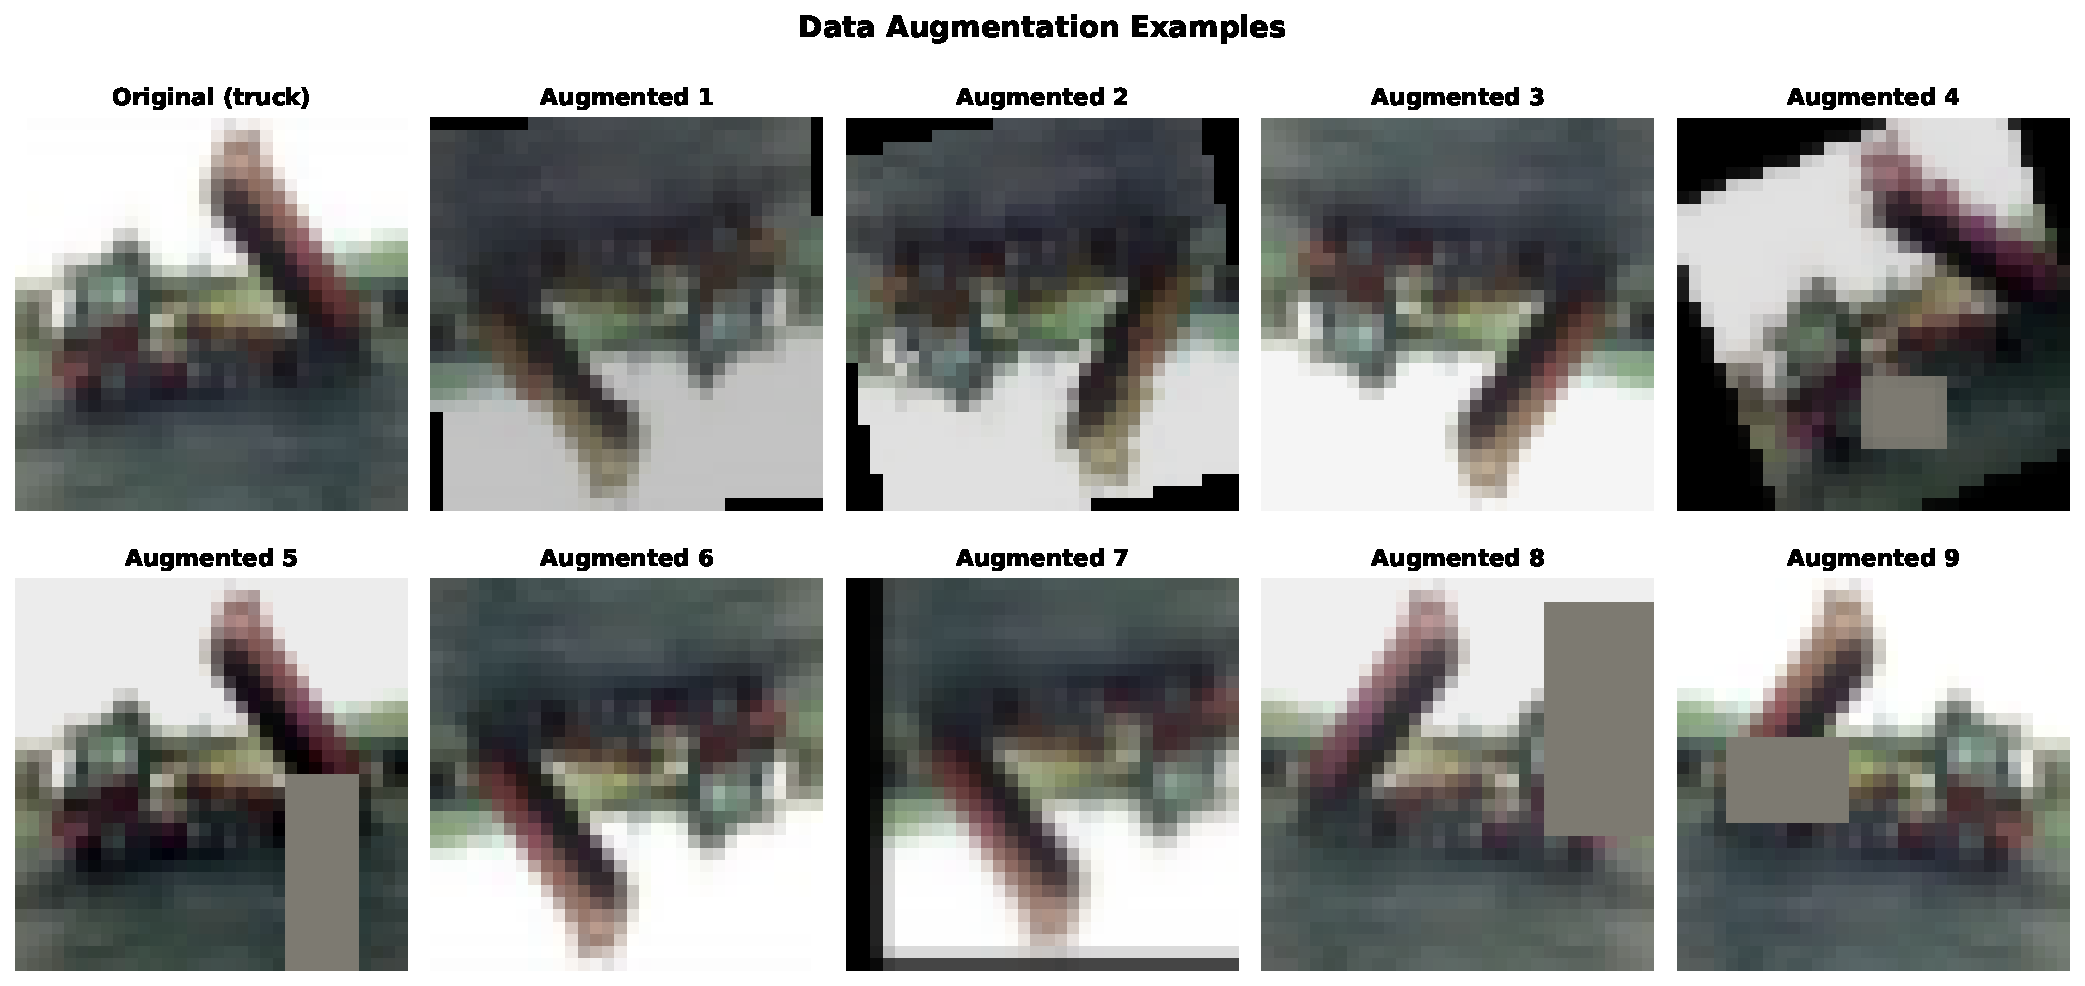
\includegraphics[width=0.9\textwidth]{../figures/data_exploration_augmentation.pdf}
  \caption{Data augmentation examples using the full augmentation pipeline. The original image (left) is followed by nine randomly augmented versions, demonstrating variations in colour, geometry, and local erasing.}
  \label{fig:augmentation}
\end{figure}


\subsection{LeNet-5}\label{subsec:lenet}

The LeNet-5 architecture \citep{lecun1998gradient} follows the pattern conv-pool-conv-pool-fc-fc-fc. 
Our implementation, defined in \texttt{LeNet()} in \texttt{my\_model.py}, 
adapts the original for 32$\times$32 RGB inputs: 
the first convolutional layer takes 3 input channels and produces 6 feature maps with a 5$\times$5 kernel, 
followed by 2$\times$2 max-pooling; the second convolutional layer maps 6 channels to 16, 
again with a 5$\times$5 kernel and 2$\times$2 pooling; 
three fully-connected layers ($400 \to 120$, $120 \to 84$, $84 \to 10$) perform the final classification. 
The model has approximately 62\,000 trainable parameters, 
making it prone to overfitting on CIFAR-10 despite its suitability for simpler tasks.


\subsection{MyCNN}\label{subsec:mycnn}

MyCNN is a ResNet-18 variant modified for 32$\times$32 inputs. 
The architecture, defined in \texttt{MyCNN()} in \texttt{my\_model.py}, 
makes three key adaptations: 
(1) the initial 7$\times$7 convolution is replaced with a 3$\times$3 convolution (stride 1, padding 1) 
to preserve spatial resolution on small inputs; 
(2) the initial max-pooling layer is removed; 
(3) the final fully-connected layer is adjusted to output 10 classes. 
The network contains four residual stages (each consisting of two BasicBlocks) 
with channel dimensions $[64, 128, 256, 512]$, adaptive average pooling, 
and approximately 11.17M trainable parameters. 
Each BasicBlock applies two 3$\times$3 convolutions with batch normalisation 
and a skip connection that shortcuts the gradient flow \citep{he2016deep}.


\section{Experiments}\label{sec:experiments}

All experiments use a consistent training pipeline: 
SGD with Nesterov momentum ($0.9$), a cosine annealing scheduler with linear warm-up (5 epochs) 
and decaying restarts, gradient clipping (max norm 1.0), and early stopping with patience 16 (64 for MyCNN).
Training is performed on an NVIDIA GeForce RTX~4090 GPU.

\subsection{Task 1: LeNet-5 Baseline}\label{subsec:task-1}

The baseline LeNet-5 is trained with a learning rate of $5\times10^{-3}$, 
no weight decay, no label smoothing, and a batch size of 64. 
The cosine annealing scheduler uses $T_0 = 48$ (first restart period), $T_{\text{mult}} = 1$, 
and $\text{cycle\_decay} = 0.05$, meaning each restart begins at 5\% of the initial peak learning rate.

As shown in Figure~\ref{fig:baseline-loss}, 
the training loss decreases monotonically from 2.28 to 0.78 over 64 epochs, 
while the validation accuracy fluctuates significantly and converges around 67\%. 
This gap between training loss and validation performance is a clear signature of overfitting: 
the model's limited capacity (~62K parameters) forces it to memorise the training set 
rather than extracting transferable features. 
Early stopping is not triggered because the validation accuracy shows small, 
gradual improvements throughout training.

\begin{figure}[tbp]
  \centering
  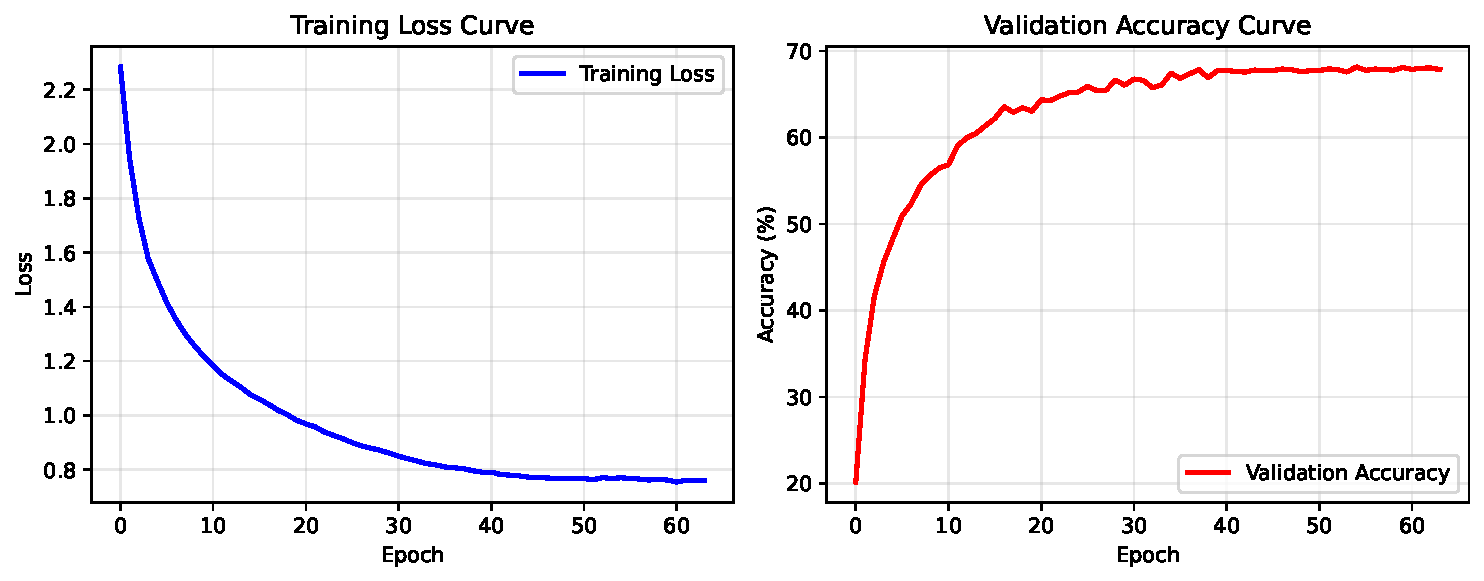
\includegraphics[width=\textwidth]{../figures/lenet_baseline_loss_curve.pdf}
  \caption{LeNet-5 baseline: training loss and validation accuracy over 64 epochs. The training loss decreases smoothly and consistently, but the validation accuracy plateaus near 67\%, indicating that the model is memorising training patterns rather than learning generalisable features.}
  \label{fig:baseline-loss}
\end{figure}

The confusion matrix (Figure~\ref{fig:baseline-confusion}) reveals that the baseline model 
is most confused among semantically similar animal classes: bird, cat, deer, and dog 
are frequently misclassified as each other. 
In contrast, vehicle classes (ship, truck, automobile) achieve substantially higher per-class accuracy. 
The worst per-class F1 score is for cat (0.4824) and the best for ship (0.8014).

\begin{figure}[tbp]
  \centering
  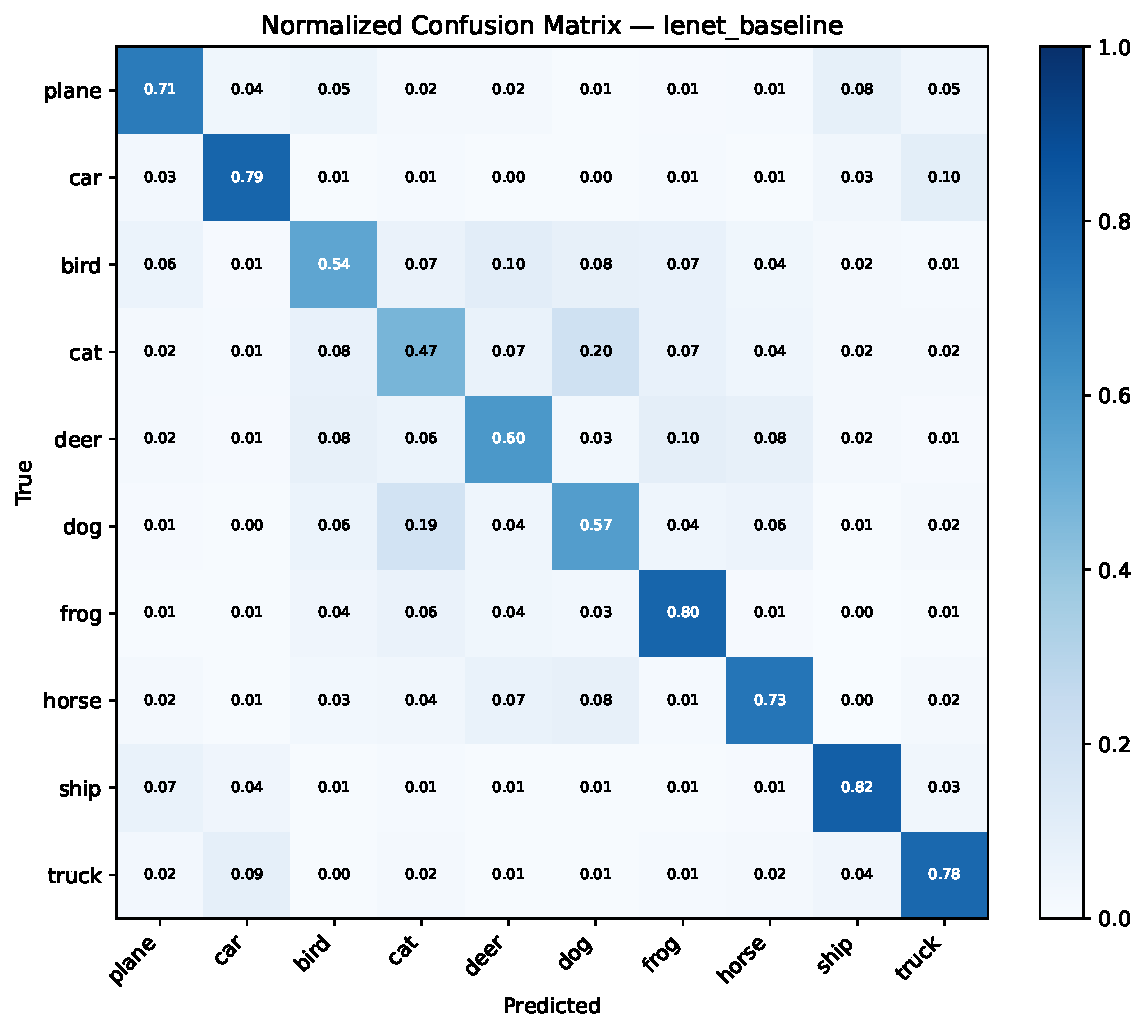
\includegraphics[width=\textwidth]{../figures/lenet_baseline_confusion_matrix.pdf}
  \caption{Normalised confusion matrix for the baseline LeNet-5 on the CIFAR-10 test set. The model is most confused between visually similar categories: bird, cat, deer, and dog, while performing well on ship, truck, and automobile.}
  \label{fig:baseline-confusion}
\end{figure}

The reliability diagram (Figure~\ref{fig:baseline-reliability}) shows that the baseline model 
tends to be overconfident in the low-to-mid confidence range, 
with an expected calibration error (ECE) of 0.0302. 
This overconfidence is typical of unregularised neural networks.

\begin{figure}[tbp]
  \centering
  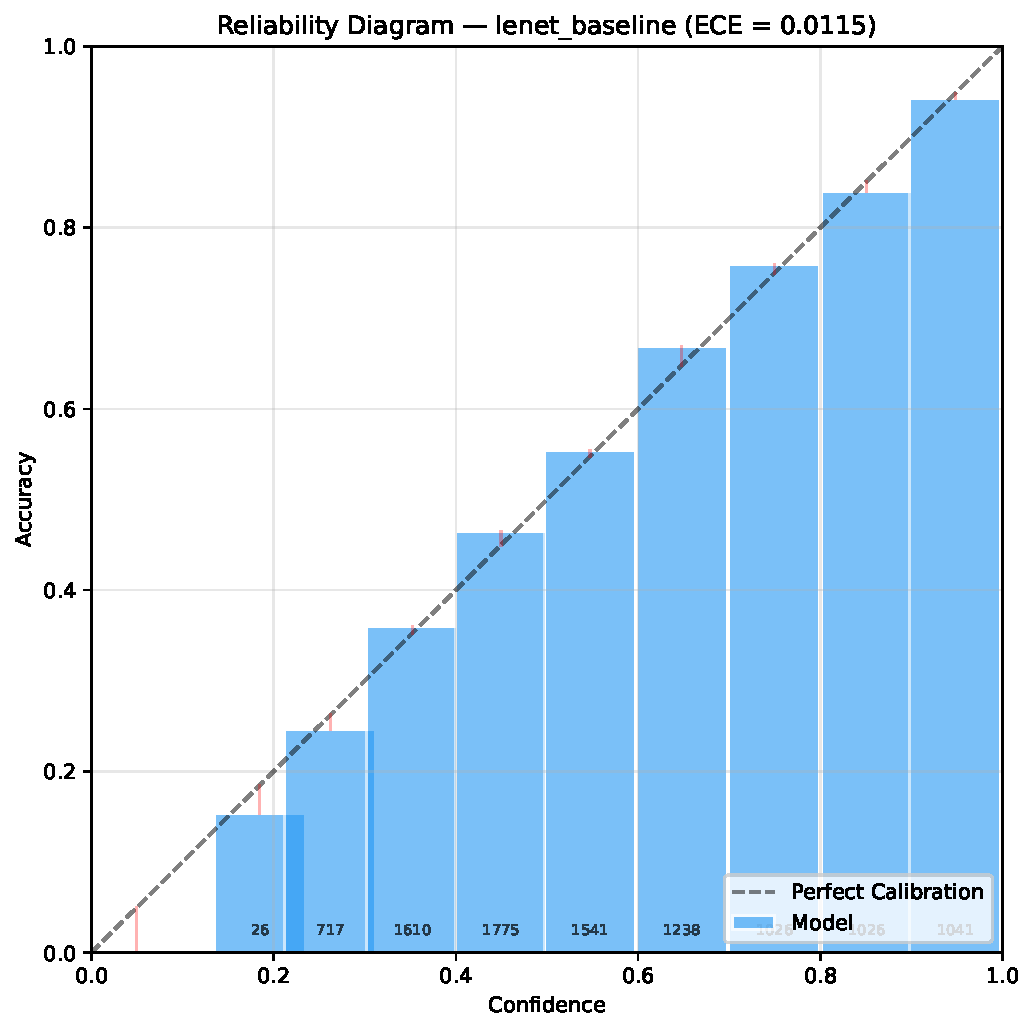
\includegraphics[width=\textwidth]{../figures/lenet_baseline_reliability_diagram.pdf}
  \caption{Reliability diagram for the baseline LeNet-5. The model overestimates its certainty in the low-confidence regime (bars below the diagonal), yielding an ECE of 0.0302. Bin counts are annotated at the bottom.}
  \label{fig:baseline-reliability}
\end{figure}

The final test accuracy is 68.02\%, 
which serves as the reference point for the regularisation and tuning experiments that follow.


\subsection{Task 2: Regularization}\label{subsec:task-2}

To mitigate the overfitting observed in Task~1, 
we introduce two regularisation techniques: Dropout and L2 weight decay. 
A Dropout layer with rate $p = 0.1$ is inserted between the first and second fully-connected layers of LeNet-5, 
and the SGD optimiser is configured with a weight decay of $1\times10^{-4}$. 
All other hyperparameters are kept identical to the baseline experiment.

Table~\ref{tab:task1-vs-task2} compares the baseline and regularised models. 
The regularised model achieves a lower test accuracy (65.01\% vs. 68.02\%), 
which is consistent with the limited-capacity hypothesis: 
for a small network with only 62K parameters, Dropout discards too many representational resources, 
causing underfitting rather than improving generalisation. 
The training loss also remains slightly higher (0.8304 vs. 0.7856), 
confirming that the model struggles to fit the training data.

\begin{table}[t]
  \centering
  \caption{Comparison of baseline and regularised LeNet-5. While regularisation improves calibration (lower ECE), it reduces test accuracy due to the limited capacity of the small network.}
  \label{tab:task1-vs-task2}
  \begin{tabular}{lccccc}
    \toprule
    Model & Train Loss & Test Acc. (\%) & ECE & Best F1 & Worst F1 \\
    \midrule
    Baseline LeNet-5 & 0.7856 & 68.02 & 0.0302 & ship (0.8014) & cat (0.4824) \\
    Regularised LeNet-5 & 0.8304 & 65.01 & 0.0194 & ship (0.7724) & cat (0.4726) \\
    \bottomrule
  \end{tabular}
\end{table}


The positive outcome of regularisation is improved calibration. 
The ECE decreases from 0.0302 to 0.0194, 
and the reliability diagram shows that the regularised model's confidence better aligns with its accuracy. 
This is further supported by Monte Carlo (MC) Dropout uncertainty estimates (see Figure~\ref{fig:mc-dropout}): 
the average predictive variance for incorrect predictions (0.0123) 
is higher than for correct predictions (0.0099), 
indicating that the model's uncertainty increases when it is about to make a mistake.

\begin{figure}[tbp]
  \centering
  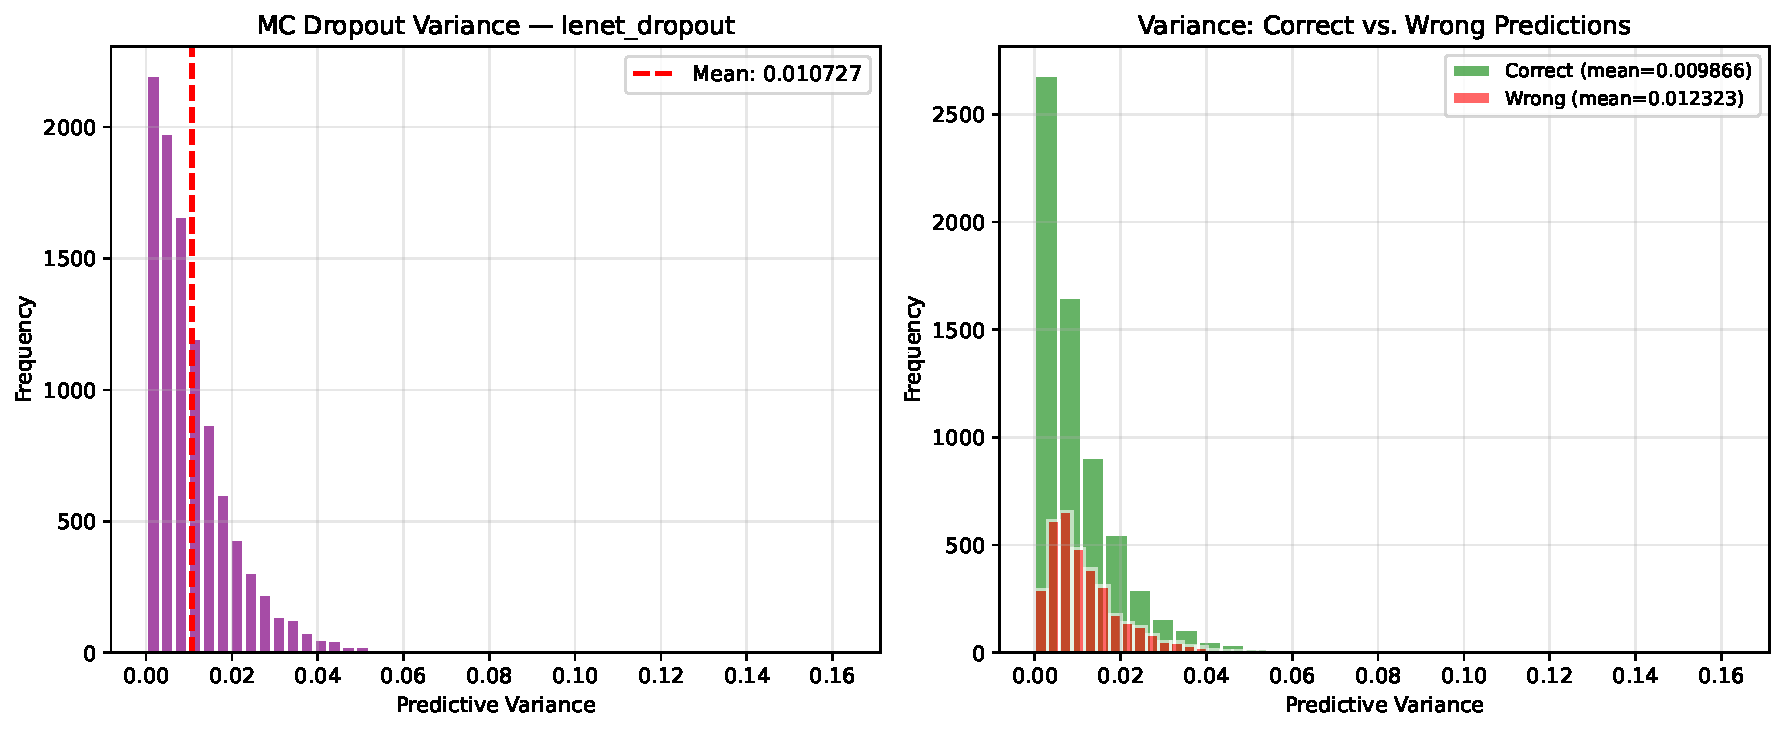
\includegraphics[width=\textwidth]{../figures/lenet_dropout_mc_dropout_variance.pdf}
  \caption{MC Dropout variance analysis for the regularised LeNet-5. Left: histogram of predictive variances across all test samples (mean = 0.0107). Right: variance split by prediction correctness; incorrect predictions (red, mean = 0.0123) exhibit higher variance than correct ones (green, mean = 0.0099), suggesting that model uncertainty correlates with error.}
  \label{fig:mc-dropout}
\end{figure}


\subsection{Task 3: Hyperparameter Tuning}\label{subsec:task-3}

We conduct a 4-factor grid search over learning rate, 
weight decay, label smoothing, and batch size, with the following values:
\begin{itemize}
  \item \textbf{Learning rate}: \{0.001, 0.005, 0.01\}
  \item \textbf{Weight decay}: \{0, $1\times10^{-4}$, $1\times10^{-3}$\}
  \item \textbf{Label smoothing}: \{0, 0.1\}
  \item \textbf{Batch size}: \{4, 16, 64\}
\end{itemize}
This yields $3 \times 3 \times 2 \times 3 = 54$ experiments, 
each using LeNet-5 with the same cosine annealing scheduler and early stopping configuration as the baseline. 
Experiments are executed in parallel using 10 concurrent worker processes.

The best combination (learning rate $10^{-2}$, weight decay $10^{-3}$, label smoothing 0.1, batch size 16) 
achieves a test accuracy of 71.40\%, representing a 3.38 percentage point improvement over the baseline.
Top-5 hyperparameter combinations by test accuracy are listed in Table~\ref{tab:task3-top5}.

\begin{table}[t]
  \centering
  \caption{Top-5 hyperparameter combinations by test accuracy from the 54-experiment grid search.}
  \label{tab:task3-top5}
  \begin{tabular}{ccccc}
    \toprule
    LR & WD & LS & BS & Test Acc. (\%) \\
    \midrule
    0.01  & $1\times10^{-3}$ & 0.1 & 16 & 71.40 \\
    0.01  & $1\times10^{-3}$ & 0.0 & 16 & 70.96 \\
    0.005 & $1\times10^{-4}$ & 0.1 &  4 & 70.93 \\
    0.01  & $1\times10^{-4}$ & 0.0 &  4 & 70.84 \\
    0.01  & $1\times10^{-3}$ & 0.1 & 64 & 70.57 \\
    \bottomrule
  \end{tabular}
\end{table}

The marginal effect analysis (Figure~\ref{fig:hyperparameter-effects}) reveals the following patterns:

\begin{itemize}
  \item \textbf{Learning rate}: Both $10^{-2}$ and $5\times10^{-3}$ substantially outperform $10^{-3}$ in terms of both the mean and variance of test accuracy.
  \item \textbf{Weight decay}: A moderate penalty of $10^{-4}$ yields the highest mean accuracy; zero weight decay is second, and an aggressive penalty of $10^{-3}$ is detrimental, consistent with the underfitting observed in Task~2.
  \item \textbf{Label smoothing}: A smoothing factor of 0.1 consistently improves mean accuracy over no smoothing, with comparable variance.
  \item \textbf{Batch size}: Smaller batches (4) achieve the highest mean accuracy, followed by 16 and then 64. Smaller batches introduce gradient noise that acts as an implicit regulariser.
\end{itemize}

\begin{figure}[tbp]
  \centering
  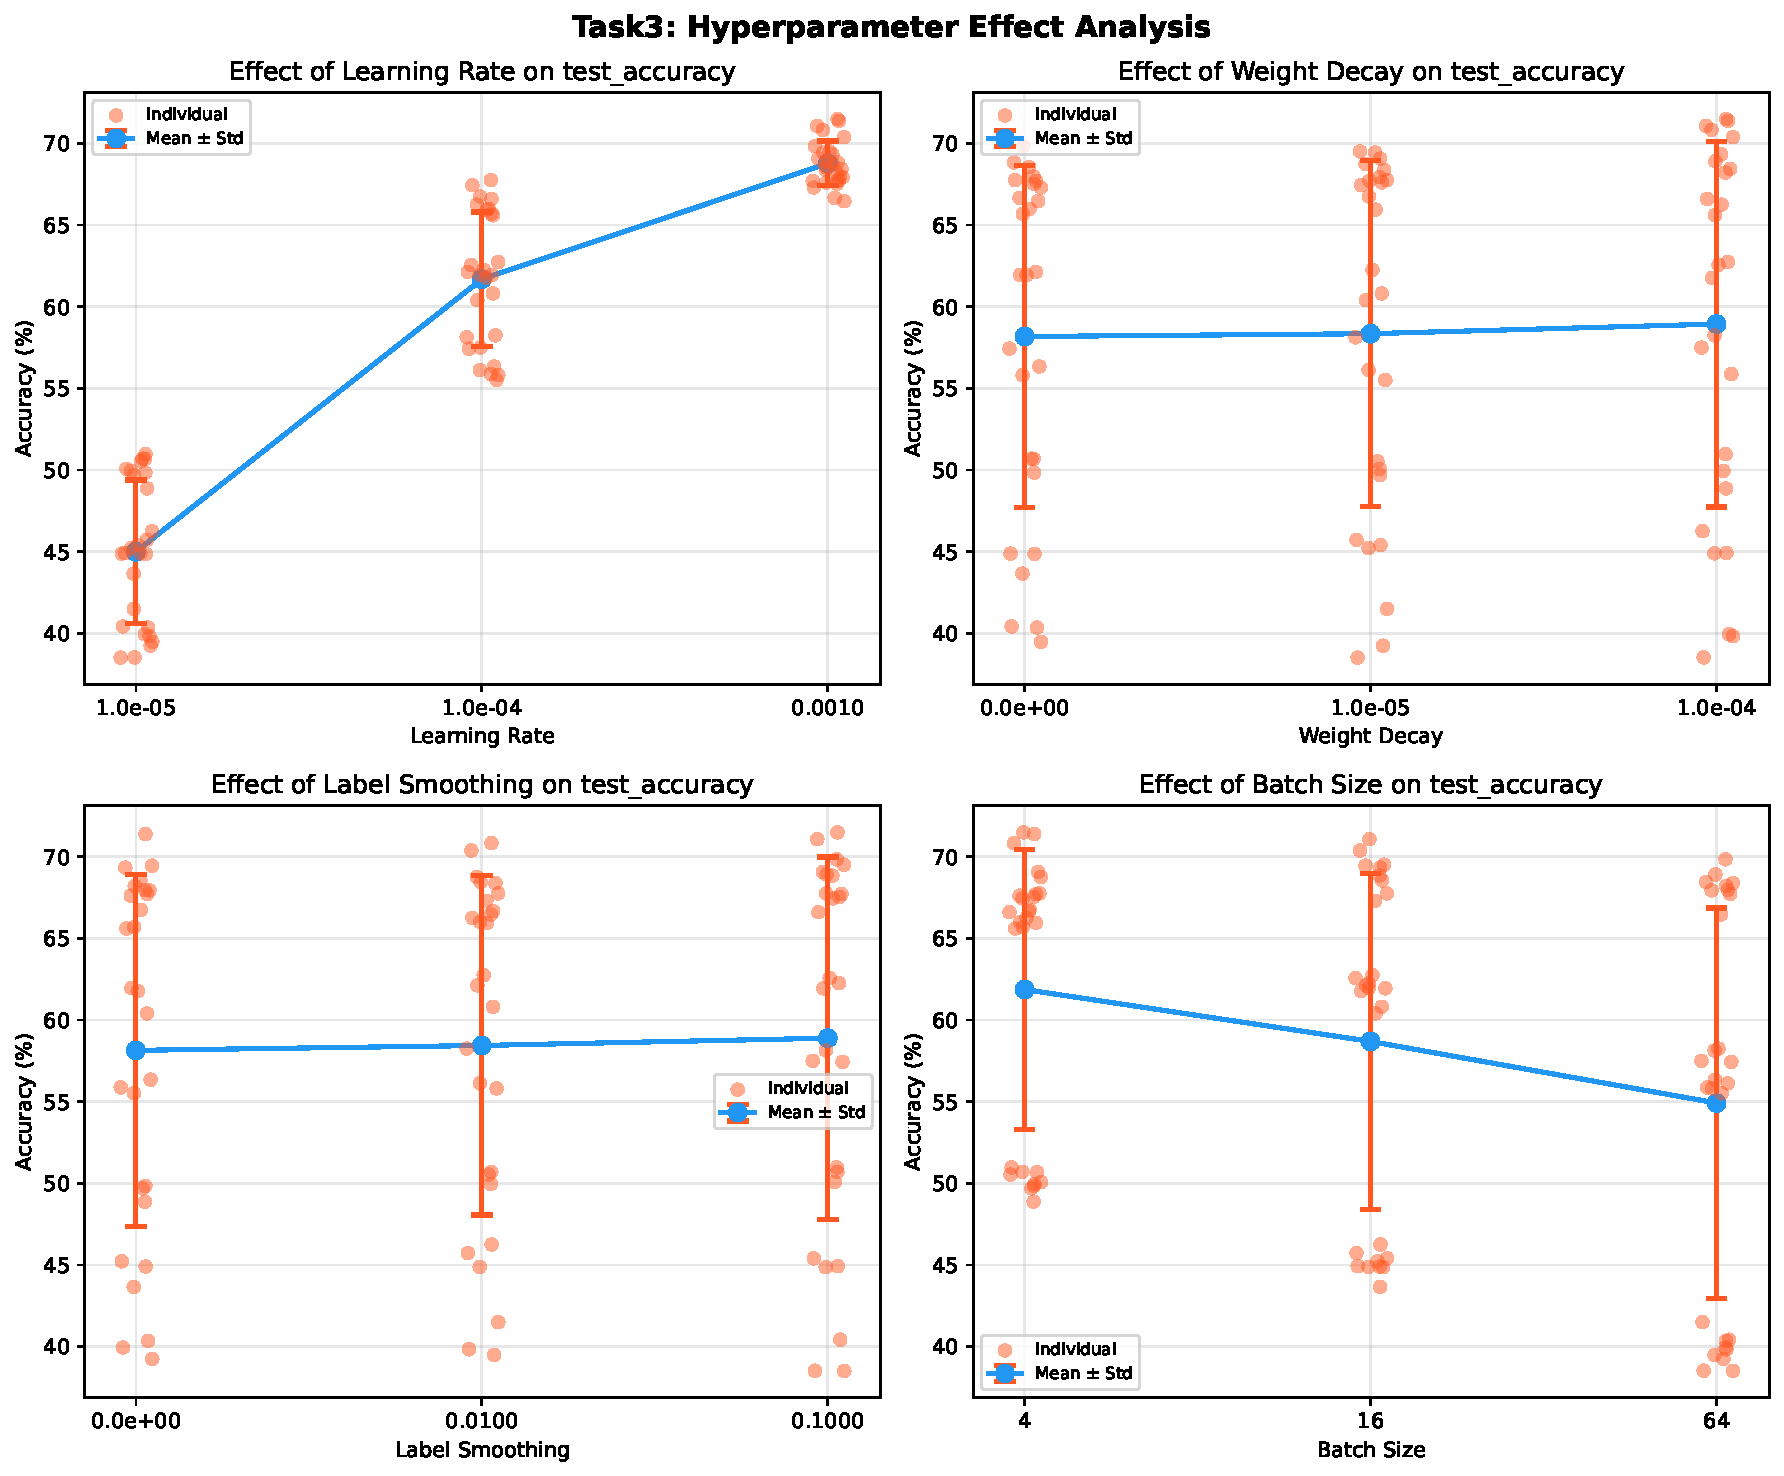
\includegraphics[width=\textwidth]{../figures/task3_hyperparameter_effects.pdf}
  \caption{Marginal effect of each hyperparameter on test accuracy across the 54-experiment grid. Dots show individual experiment results; lines connect group means with $\pm 1$ standard deviation error bars.}
  \label{fig:hyperparameter-effects}
\end{figure}

The LR $\times$ BS interaction (Figure~\ref{fig:lr-bs-interaction}) confirms a known heuristic: 
larger batch sizes require larger learning rates. 
At LR $= 10^{-3}$, batch size 4 clearly outperforms 16 and 64. 
At batch sizes 16 and 64, the learning rate of $10^{-2}$ achieves the best results, 
suggesting that increasing the learning rate compensates for the reduced gradient noise of larger batches.

\begin{figure}[tbp]
  \centering
  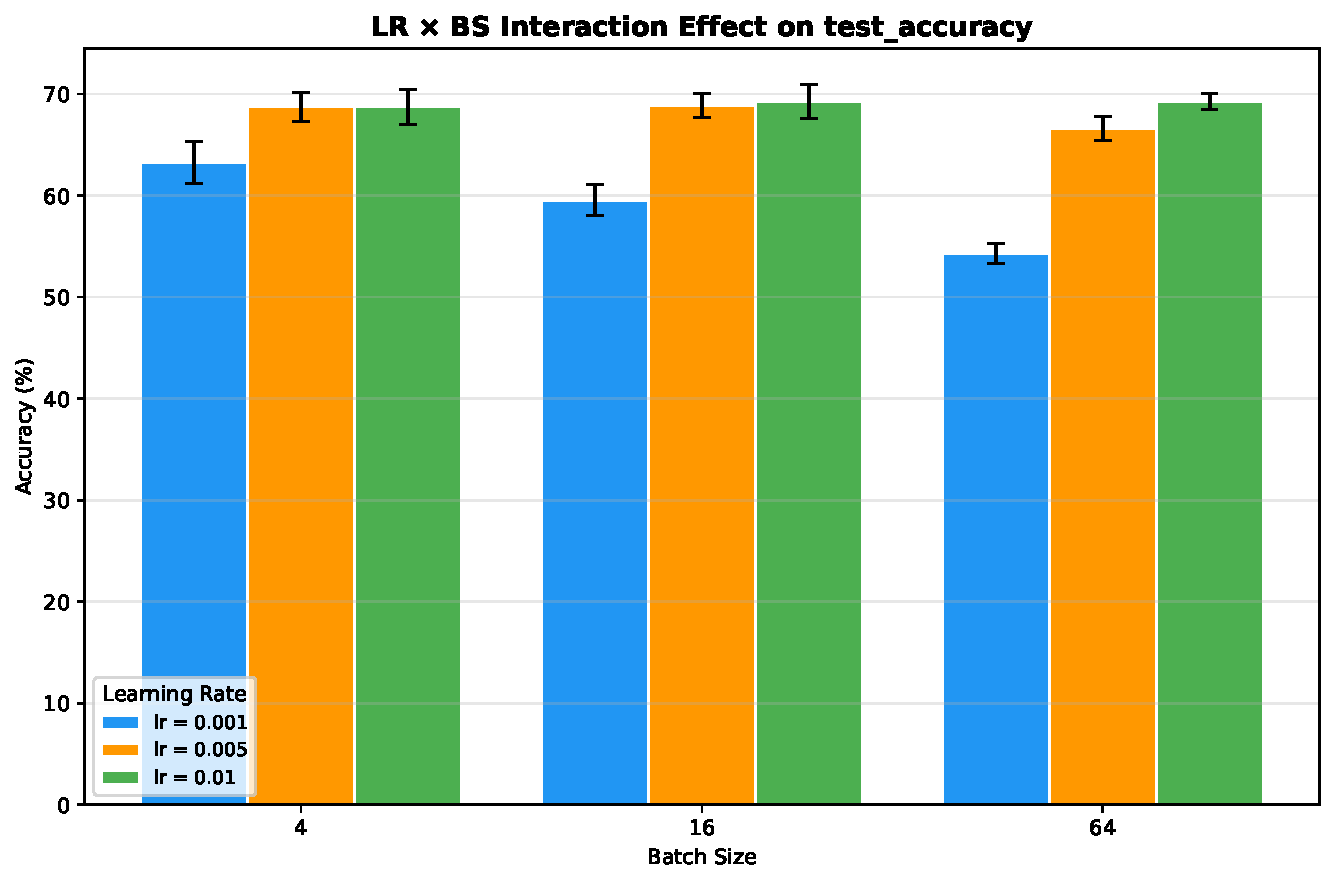
\includegraphics[width=\textwidth]{../figures/task3_lr_bs_interaction.pdf}
  \caption{LR $\times$ BS interaction effects on test accuracy. At low learning rates, smaller batches perform best; at larger batch sizes, higher learning rates are necessary to maintain effective step sizes.}
  \label{fig:lr-bs-interaction}
\end{figure}

\subsection{Task 4: Modern CNN (MyCNN)}\label{subsec:task-4}

MyCNN is trained with a learning rate of $10^{-1}$, weight decay $5\times10^{-4}$, 
label smoothing $0.05$, and batch size 128. 
It uses the full augmentation pipeline described in Section~\ref{subsec:data-augmentation} 
and a cosine annealing scheduler with $T_0 = 80$, $\text{cycle\_decay} = 0.1$, 
and an extended early stopping patience of 64 epochs. Training runs for up to 320 epochs.

The training dynamics (Figure~\ref{fig:mycnn-loss}) show a rapid initial drop in loss 
followed by a long tail of gradual improvement. 
A noticeable spike around epoch~80 corresponds to the first cosine annealing restart, 
where the learning rate jumps from its minimum back to the cycle peak (10\% of the initial LR due to $\text{cycle\_decay} = 0.1$). 
The validation accuracy follows a high-variance trajectory during early training but stabilises above 95\% after approximately 200 epochs.

\begin{figure}[tbp]
  \centering
  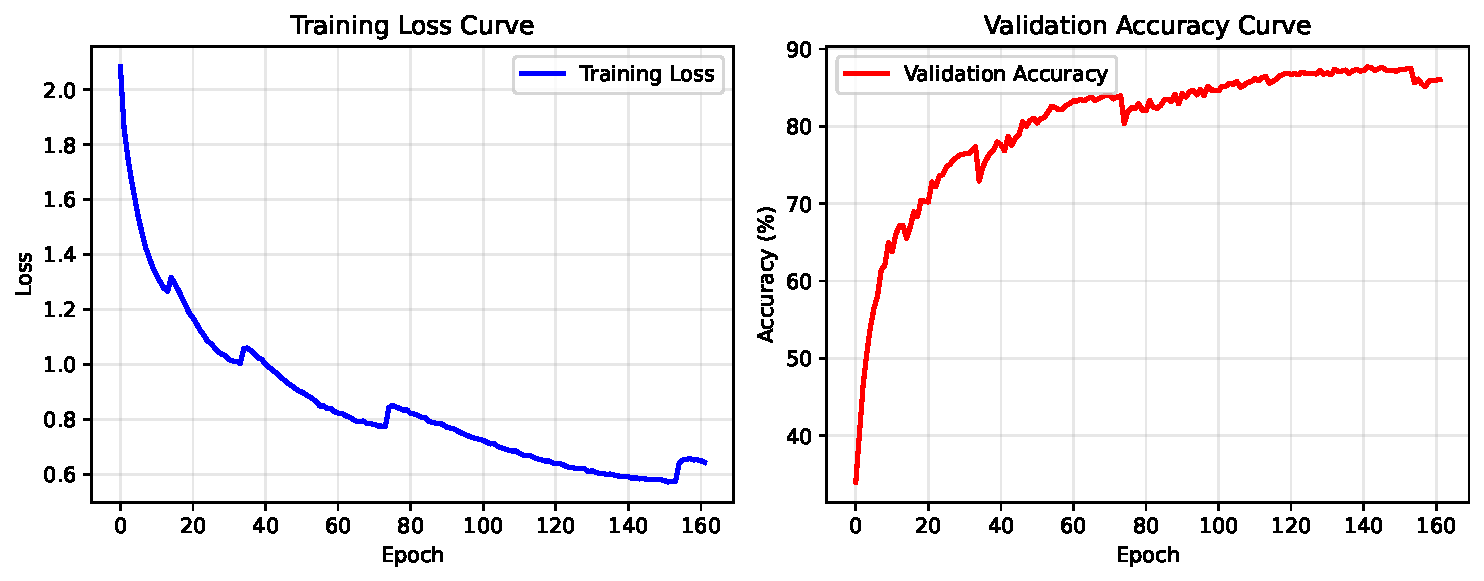
\includegraphics[width=\textwidth]{../figures/mycnn_loss_curve.pdf}
  \caption{MyCNN training loss and validation accuracy over 278 epochs. Training loss decreases rapidly in the first few epochs before entering a regime of slower improvement. A spike around epoch~80 coincides with the first cosine annealing restart, after which the loss decreases further. The validation accuracy stabilises above 95\% after approximately 200 epochs.}
  \label{fig:mycnn-loss}
\end{figure}


MyCNN achieves a best validation accuracy of 95.84\% and a test accuracy of 95.04\% (Table~\ref{tab:final-comparison}). 
This represents a substantial improvement of over 27 percentage points compared to the best LeNet-5 configuration from Task~3, 
attributable to the combination of deeper architecture (11.17M vs. 62K parameters), 
stronger data augmentation, and carefully tuned hyperparameters.

\begin{table}[t]
  \centering
  \caption{Full comparison across all four experimental tasks. MyCNN achieves a dramatic improvement over all LeNet-5 variants.}
  \label{tab:final-comparison}
  \begin{tabular}{lccccc}
    \toprule
    Model & Params & Test Acc. (\%) & ECE & Best F1 & Worst F1 \\
    \midrule
    LeNet-5 baseline & 62K & 68.02 & 0.0302 & ship (0.8014) & cat (0.4824) \\
    LeNet-5 regularised & 62K & 65.01 & 0.0194 & ship (0.7724) & cat (0.4726) \\
    LeNet-5 tuned (best) & 62K & 71.40 & 0.7181 & car (0.8413) & cat (0.5430) \\
    MyCNN (ResNet-18) & 11.17M & 95.04 & 0.0394 & car (0.9727) & cat (0.8894) \\
    \bottomrule
  \end{tabular}
\end{table}

The confusion matrix (Figure~\ref{fig:mycnn-confusion}) shows that MyCNN primarily confuses cat with dog, 
which is expected given the visual similarity between these two classes. 
All other classes are robustly distinguished, with most diagonal entries exceeding 0.95. 
The per-class F1 scores are uniformly high, with car achieving the best (0.9727) and cat the worst (0.8894).

\begin{figure}[tbp]
  \centering
  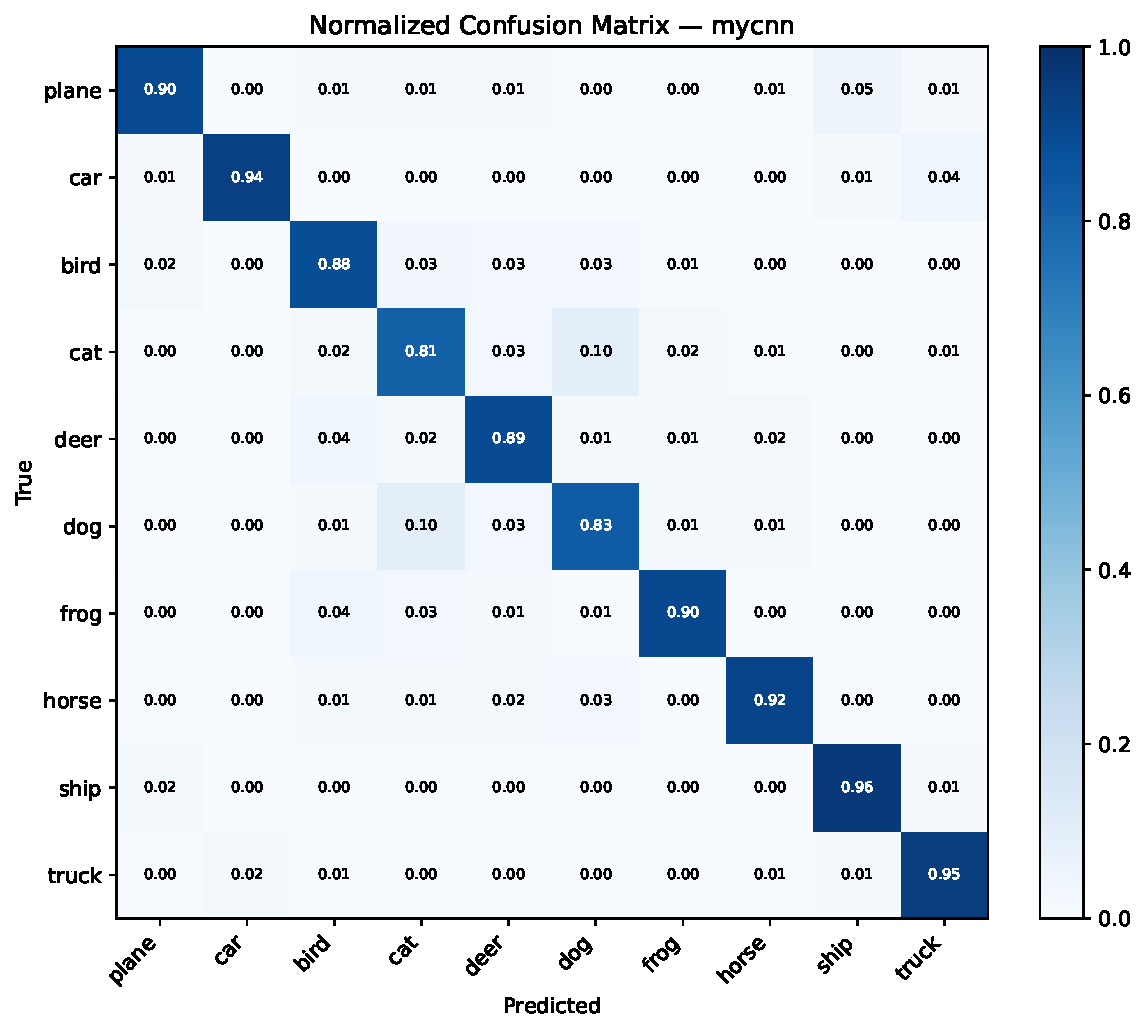
\includegraphics[width=\textwidth]{../figures/mycnn_confusion_matrix.pdf}
  \caption{Normalised confusion matrix for MyCNN on the CIFAR-10 test set. The model primarily confuses cat with dog; all other classes are reliably distinguished.}
  \label{fig:mycnn-confusion}
\end{figure}

The reliability diagram (Figure~\ref{fig:mycnn-reliability}) reveals that MyCNN overestimates certainty 
in low-confidence predictions but approaches near-perfect calibration at high confidence levels. 
The ECE of 0.0394 is higher than that of the regularised LeNet-5, 
likely because the model's strong predictive performance concentrates most predictions in the highest confidence bin.

\begin{figure}[tbp]
  \centering
  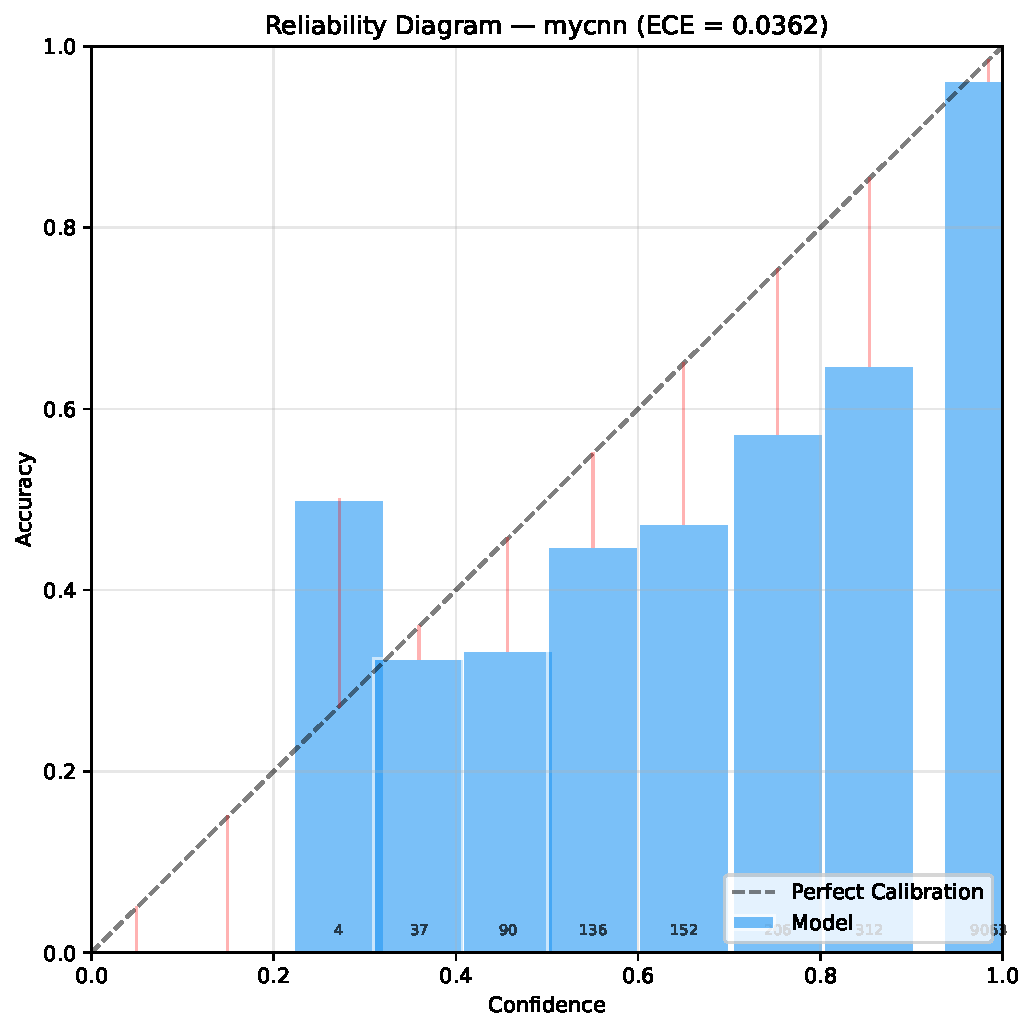
\includegraphics[width=\textwidth]{../figures/mycnn_reliability_diagram.pdf}
  \caption{Reliability diagram for MyCNN. The model overestimates certainty at low confidence but achieves near-perfect calibration at high confidence. ECE = 0.0394. Most samples fall into the highest confidence bin (annotated count: 9600+).}
  \label{fig:mycnn-reliability}
\end{figure}

\section{Conclusion}\label{sec:conclusion}

This report systematically evaluated CNN design and training on the CIFAR-10 benchmark across four experimental tasks. 
The baseline LeNet-5 achieved 68.02\% test accuracy but exhibited clear overfitting, 
with a decreasing training loss that did not translate into high test accuracy. 
Introducing L2 regularisation and Dropout improved model calibration (ECE reduced from 0.0302 to 0.0194) 
but reduced test accuracy to 65.01\%, 
confirming that aggressive regularisation harms small-capacity networks by inducing underfitting. 
A 54-experiment hyperparameter grid search revealed that learning rate has the largest marginal effect on accuracy, 
while batch size interacts systematically with learning rate such that larger batches require higher learning rates. 
The optimal hyperparameter combination achieved 71.40\% test accuracy. 
Finally, MyCNN -- a ResNet-18 variant adapted for 32$\times$32 inputs -- reached 95.04\% test accuracy, 
demonstrating the dramatic impact of architectural capacity and modern training techniques.

Several limitations should be acknowledged. 
The hyperparameter grid search, while covering four factors, 
used a relatively small number of values per factor and did not explore interactions beyond LR $\times$ BS. 
The modern CNN investigation was limited to a single architecture; 
exploring other designs (VGG, WideResNet, DenseNet) would provide a more comprehensive picture. 
Training was also limited to a single seed per configuration. 
Future work could extend this study by incorporating learning rate range tests for determining optimal LR bounds, 
Bayesian hyperparameter optimisation, and systematic ablation studies of each architectural component in MyCNN.

\bibliography{references}

\end{document}